\begin{center}
	$ t=t_0 $:
\begin{center}
	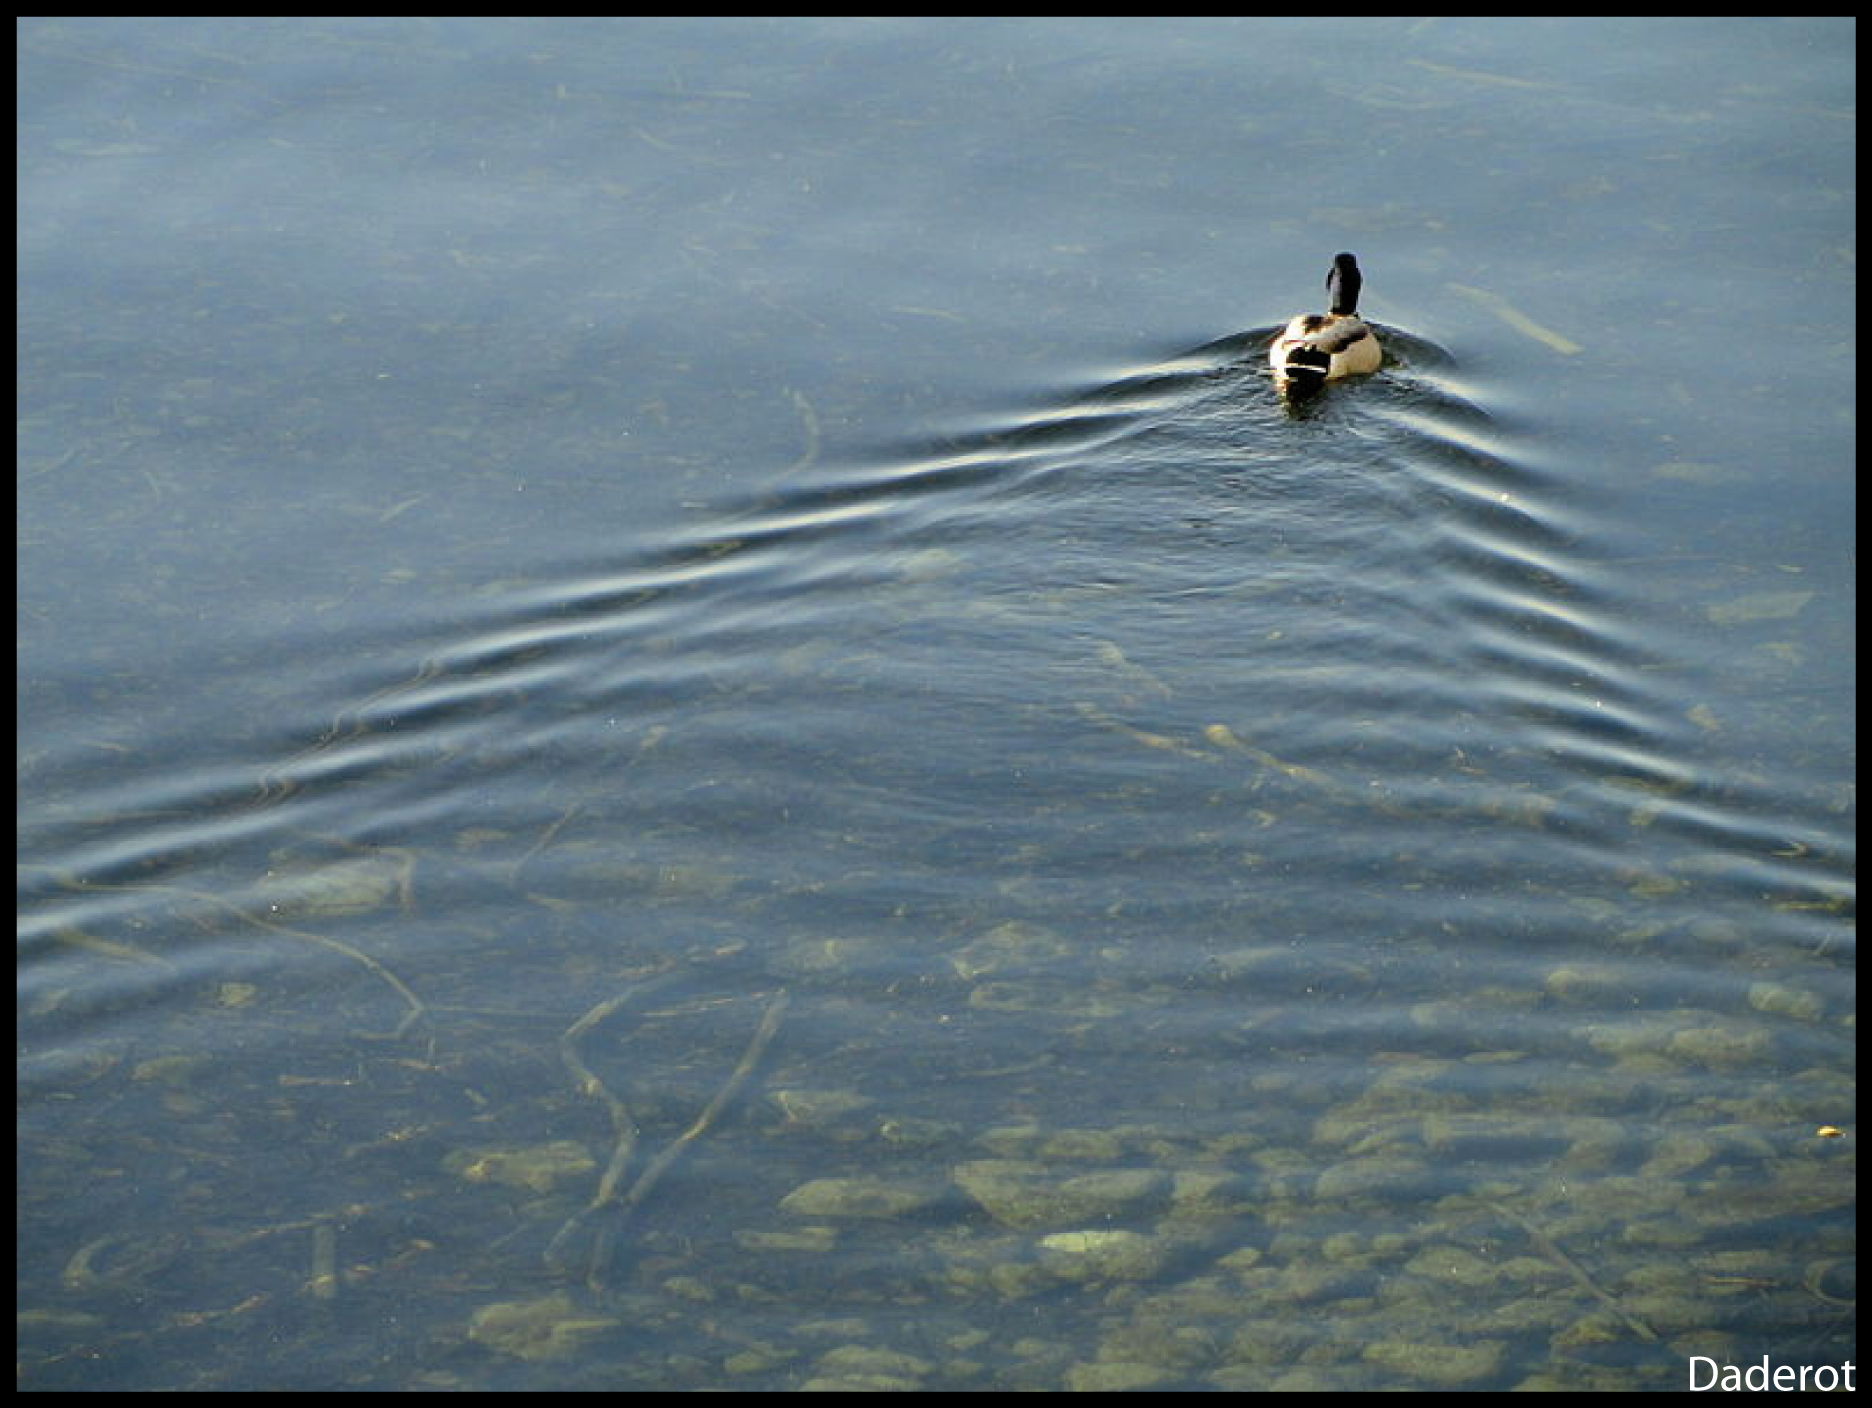
\includegraphics[width=0.5\linewidth]{skizzen/19/19B02}
\end{center}
Räumliche Periodizität

\HL

$ \vec{r} = \vec{r}_0 $
\begin{center}
	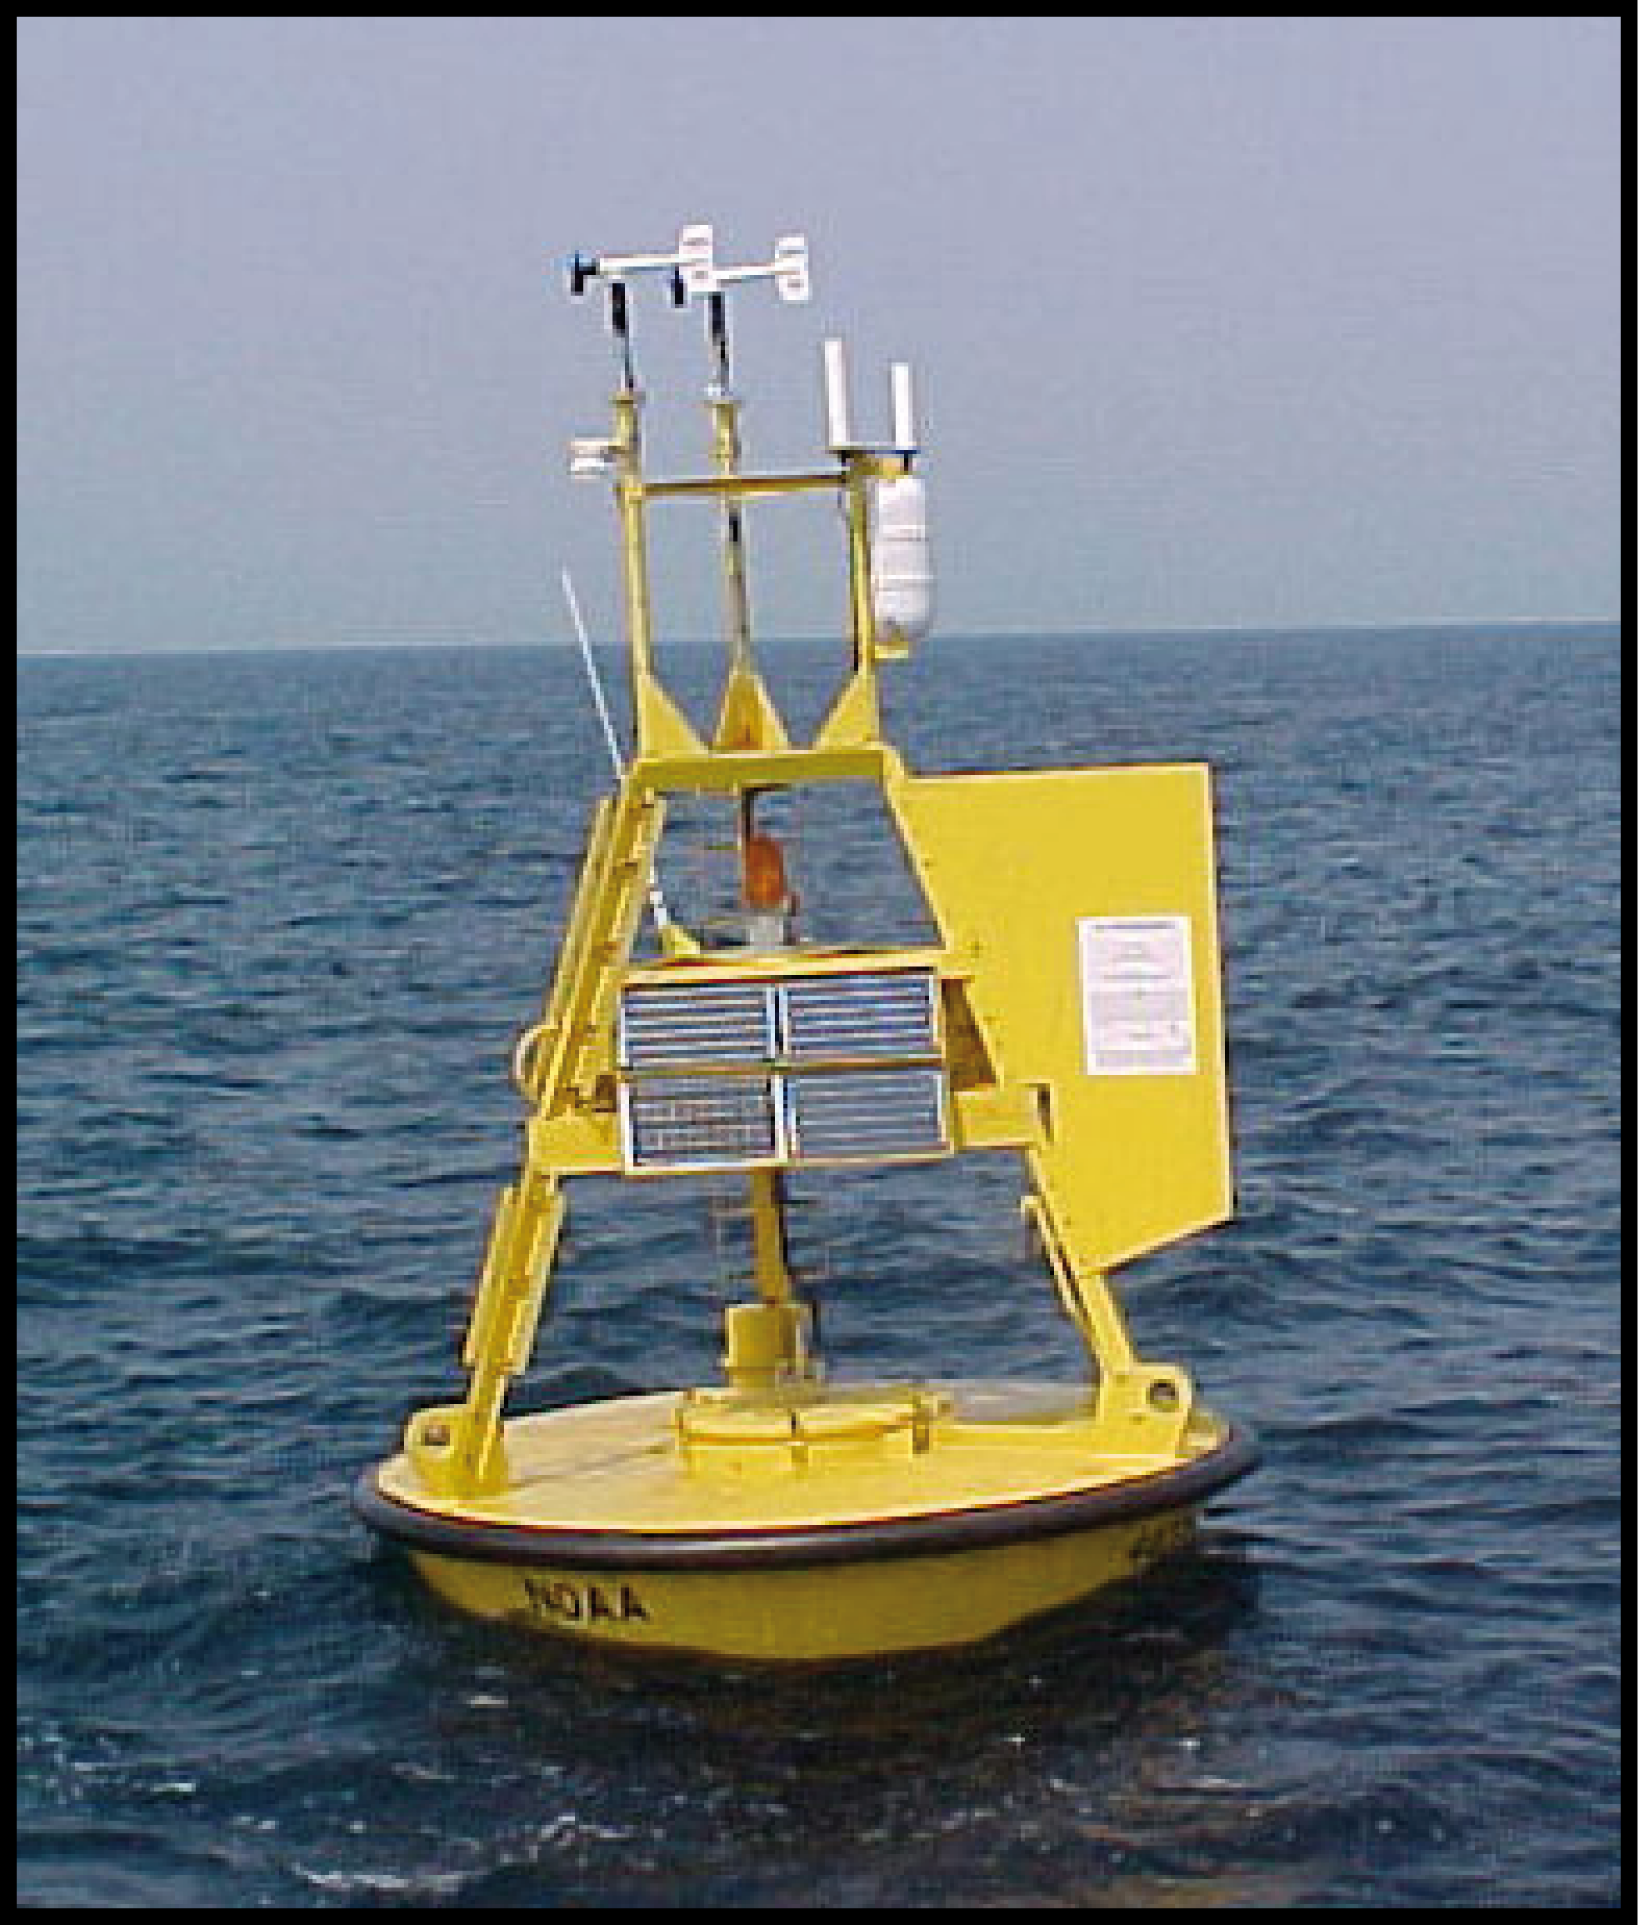
\includegraphics[width=0.5\linewidth]{skizzen/19/19B01}
\end{center}
zeitliche Periodizität
\end{center}

Welle: Zeitlich und räumlich periodische Auslenkung einer Zustandsänderung.\\
$ \Rightarrow $ Energie- und Impulstransport \underline{ohne} Materialtransport!\\
\paragraph{Experiment} \hfill \\
Einmalige Störung
\begin{center}
	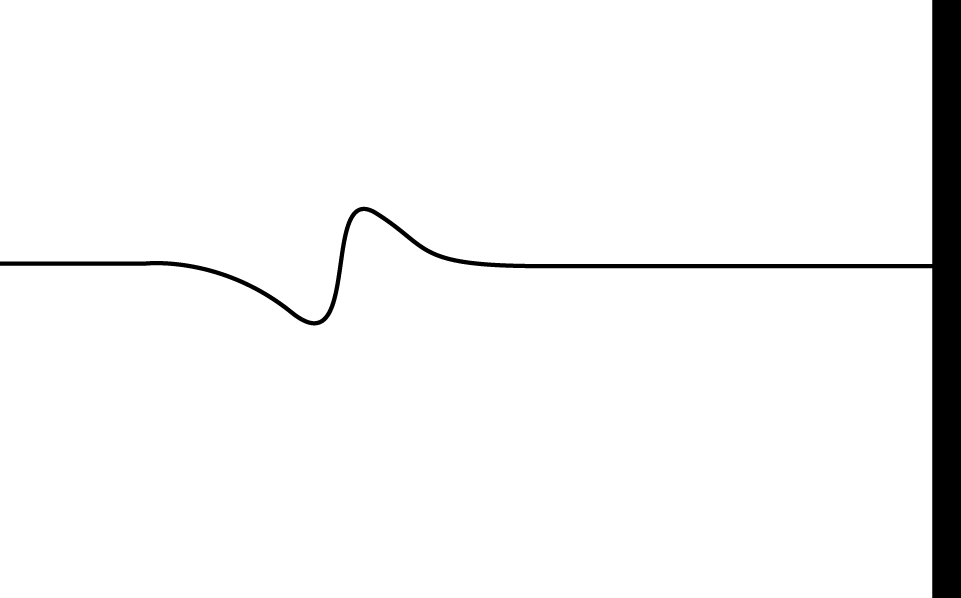
\includegraphics[width=0.5\linewidth]{skizzen/19/19B03}
	\enter
	$ \Rightarrow $ Kein periodischer Vorgang!
\end{center}

\paragraph{Experiment: WWW} \hfill \\
Periodische Erregung, Ausbreitung ohne Materialtransport!
\begin{itemize}
	\item punktförmiger Erreger: Kreiswellen
	\item linienförmiger Erreger: Ebene Welle
\end{itemize}
\paragraph{Heutz'sche Dipol} \hfill \\
Emission mit charakteristischer Abschallgeometrie
\paragraph{Verdichtungswelle ($ \Rightarrow $ "Wellenmaschine")} \hfill \\
$ \Rightarrow $ Unterschied: \underline{Transversalwelle}, \underline{Longitudinalwelle}
